\documentclass[border=3pt,tikz]{standalone}
\usepackage{physics}
\usepackage{tikz}
\usepackage[outline]{contour} % glow around text
\usetikzlibrary{calc}
%\usetikzlibrary{angles,quotes} % for pic
%\usetikzlibrary{arrows.meta}
%\usetikzlibrary{patterns}
\tikzset{>=latex} % for LaTeX arrow head
\contourlength{1.35pt}

\colorlet{xcol}{red!50!black}
\colorlet{xcol'}{green!50!black}
\colorlet{xcol''}{blue!70!black}
\colorlet{vcol}{green!60!black}
\colorlet{myred}{red!65!black}
\colorlet{mydarkred}{red!40!black}
\colorlet{mypurple}{blue!60!red!80}
\colorlet{mydarkgreen}{green!20!black}
\tikzstyle{rvec}=[->,xcol,very thick,line cap=round]
\tikzstyle{Rvec}=[->,xcol'',very thick,line cap=round]
\tikzstyle{nvec}=[->,blue!30!black,very thick,line cap=round]
\tikzstyle{vvec}=[->,vcol,very thick,line cap=round]
\tikzstyle{CM}=[mydarkred,fill=red!80!black!80]
\tikzstyle{mass}=[line width=0.6,draw=red!30!black, %rounded corners=1,
                  top color=mydarkred!30,bottom color=mydarkred!10,shading angle=30]
\tikzstyle{dark mass}=[line width=0.3,red!30!black, %rounded corners=1,
                       top color=mydarkred!40,bottom color=mydarkred!60,shading angle=30]

\def\r{0.05} % pulley small radius
\tikzset{
  pics/rotarr/.style={
    code={
      \draw[white,very thick] ({#1*cos(200)},0) arc(-200:30:{#1} and {#1/2}) --++ (125:0.1);
      \draw[->,mydarkgreen] ({#1*cos(200)},0) coordinate (W1) arc(-200:20:{#1} and {#1/2}) node[midway] (W2) {} --++ (125:0.1) coordinate (W3);
  }},
  pics/rotarr/.default=0.4,
}


\begin{document}


\def\L{1.2}    % size scale
\def\A{2.1}    % height axis above body
\def\d{3}    % distance parallel axis to CM
\def\ang{-30}  % angle connection between axes
\def\anga{72}  % angle axes
\def\bodyshape{
  ($(M)$) ellipse [x radius=2.2*\L, y radius=3*\L,rotate=-18]
}

\def\body{ % shape
  \fill[ball color=red!80!black] \bodyshape;
  \draw[line width=0.6,draw=red!30!black,fill=red!60!black!5,fill opacity=0.85]
    \bodyshape;
  %\fill[mass] \bodyshape;
}


\def\ys{0.6}     % vertical minor axis ellipse
\def\ri{0.56*\d} % small mass m_i distance from axis
\def\angi{210}   % small mass m_i polar angle
\def\dx{0.15}    % size small mass m_i


\begin{tikzpicture}
  \def\angi{240}                 % small mass m_i polar angle
  \coordinate (M) at (0,0);      % center of mass
  \coordinate (R) at (\ang:\d);  % intersection with new axis
  \path[rotate around={\ang:(R)}]
    (R) --++ (\angi:{\ri} and {\ys*\ri}) coordinate(Ri); % small mass m_i
  
  % BODY
  
  \body

  % CENTER OF MASS, MASS i and center O
  \draw[CM] (M) circle(0.09) node[above=0,left] {CM}; % center of mass point
  \draw[CM] (R) circle(0.09) node[above=0,right] {O}; % center of mass point


  % AXES
  \draw (M) --++ (\anga-180:2.2*\L) node[above left] {$b$}; % axis below
  \draw (R) --++ (\anga-180:1.7*\L) node[above=4,right=2] {$a$}; % axis below
  \fill[red!80!black] (R) circle(0.02);
  \draw (M)++(\anga:0.05) --++ (\anga:\A); % axis above
  \draw (R) --++ (\anga:1.2*\A); % axis above
  \pic[rotate=\anga-90] at ($(R)+(\anga:\A)$) {rotarr}; % rotation arrow
  \node[mydarkgreen,right=0] at (W3) {$\omega$};
  %\draw[<->] (\anga:0.55*\A) --++ (\ang:\d) % distance/radius R
  %  node[pos=0.5, above=-0.5] {\contour{white}{$\|\vb{R}\|$}};
  \draw[nvec]
  ($(R) + (\anga:1.6*\L)$) --++ (\anga:1.2*\L) node[pos=0.5,left=-0.2] {$\vb{n}$};

  %__FIRST MASS__
    \coordinate (Rs) at ($(R) + ({180+\anga}:0.5*\L)$);
    \coordinate (Ms) at ($(M) + ({180+\anga}:0.5*\L)$);
    \coordinate (Ris) at ($(Ri) + ({180+\anga}:0.5*\L)$);
      
    % VECTORS
    \node[mydarkred,right=-12,below=-2,scale=0.9] at (Ris) {$dm_2$};

    \draw[rvec] (Rs) -- ($(Rs)!0.96!(Ris)$)
      node[pos=0.5,below right=-2] {$\vb{r}_{\text{2}}$};
    
    \draw[rvec,xcol'] (Ms)++(-50:0.05) -- ($(Ms)!0.99!(Ris)$)
      node[pos=0.4,below=1] {$\vb{r'}_{\text{2}}$};
    \draw[Rvec] (Rs) -- ($(Rs)!0.99!(Ms)$)
      node[pos=0.5,above=-0.2] {$\vb{R}$};
    
    \draw[dark mass,rotate=\ang+\angi+30] % mass m_i
        (Ris)++(-45:{\dx/sqrt(2)}) to[out=95,in=-100]++
        (90:\dx) to[out=170,in=10]++
        (180:\dx) to[out=-100,in=100]++
        (-90:\dx) to[out=10,in=175]++ (0:\dx) -- cycle;



    %__SECOND MASS__
    \coordinate (shiftvec) at ($-2*(Ris)$); %the second mass is a point reflection of the first one, with respect to CM. Ris is exactly the vector from CM to dm_n_1 and we thus subtract twice this vector from Ris to get Riss.

    \coordinate (Riss) at ($ (Ris) + (shiftvec) $);

    \node[mydarkred,right=15,above=-1,scale=0.9] at (Riss) {$dm_1$};

          
    % VECTORS
    \coordinate (Rss) at ($(R) + ({\anga}:0.5*\L)$);
    \coordinate (Mss) at ($(M) + ({\anga}:0.5*\L)$);
    

    \draw[rvec] (Rss) -- ($(Rss)!0.98!(Riss)$)
      node[pos=0.5,above right=-2] {$\vb{r}_{\text{1}}$};
    
    \draw[rvec,xcol'] (Mss)++(-50:-0.05) -- ($(Mss)!0.99!(Riss)$)
      node[pos=0.6,below=1] {$\vb{r'}_{\text{1}}$};
    \draw[Rvec] (Rss) -- ($(Rss)!0.99!(Mss)$)
      node[pos=0.5,below=-0.2] {$\vb{R}$};
      
    \draw[dark mass,rotate=\ang+\angi+30] % mass m_i
        (Riss)++(-45:{\dx/sqrt(2)}) to[out=95,in=-100]++
        (90:\dx) to[out=170,in=10]++
        (180:\dx) to[out=-100,in=100]++
        (-90:\dx) to[out=10,in=175]++ (0:\dx) -- cycle;


% Dotted-dashed grayish line between the masses
\draw[black!70, dash pattern=on 2pt off 1pt on 0.5pt off 1pt] (Ris) -- (Riss);


\end{tikzpicture}

%__The 2D projection perpendicular on vector n, of the triangle that is the result of combinating the two triangles on the 3D figure
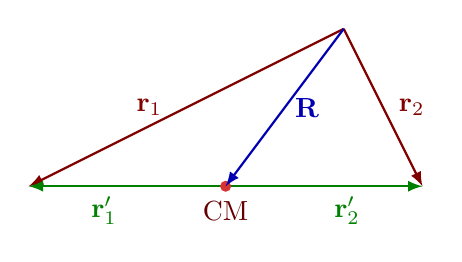
\begin{tikzpicture}[scale=1,>=latex]

% triangle points
\coordinate (Top)   at (1.5,2);   % top vertex
\coordinate (Left)  at (-2.5,0);  % left vertex
\coordinate (Right) at (2.5,0);   % right vertex
\coordinate (CM)    at (0,0);   % center of base

% triangle sides with vectors pointing away from top
\draw[xcol,thick,->] (Top) -- (Left) node[midway, left=5pt] {$\vb{r}_1$};
\draw[xcol,thick,->] (Top) -- (Right) node[midway, right=2pt] {$\vb{r}_2$};

% vectors along base from middle outward
\draw[xcol',thick,->] (CM) -- (Left) node[midway, below left] {$\vb{r}'_1$};
\draw[xcol',thick,->] (CM) -- (Right) node[midway, below right] {$\vb{r}'_2$};

% CM node
\fill[CM] (CM) circle(0.07) node[below=2pt] {CM};

% vector from top to CM
\draw[xcol'',thick,->] (Top) -- (CM) node[midway,right] {$\vb{R}$};

\end{tikzpicture}




\end{document}